\documentclass[../main.tex]{subfiles}

\graphicspath{{\subfix{../figures}}}

\begin{document}

\begin{figure*}[t!]
  \centering
  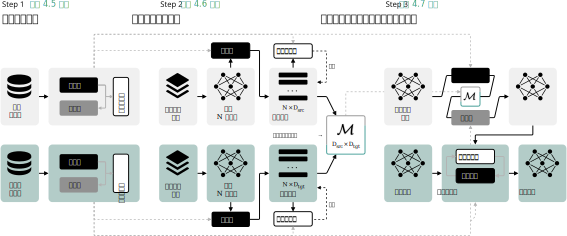
\includegraphics[width=.95\linewidth]{overview}
  \caption{
    Overview of the \OUR{} framework.
    The whole process can be decomposed to three steps:
    (1) building representations with supervised and unsupervised representation learning;
    (2) learning mapping between representations from source and target domains;
    (3) transfer historical solutions from source domain with representation model and mapping to target domain.
  }\label{fig:overview}
\end{figure*}

\section{Proposed Method}\label{sec:method}

This section presents a comprehensive description of our proposed cross-domain evolutionary transfer neural architecture search framework \OUR{}.
We begin with an overview of the entire framework, followed by in-depth discussions of its key components.
These components include building neural architecture representation, constructing cross-domain transfer mappings, and performing cross-domain evolutionary transfer for NAS\@.
Each of these elements plays a crucial role in our proposed approach to TNAS across heterogeneous search spaces.

\subsection{Overview of \OUR{}}

As shown in Fig.~\ref{fig:overview}, the entire framework of \OUR{} can be decomposed into several steps.
Initially, the neural architecture representation learner undergoes training on both the source and target domains independently.
This process aims to establish the encoding and decoding capabilities necessary for bridging the architecture space and the representation space.
Subsequently, utilizing sampling in the representation space aligned with a performance metric, the model learns the mapping between the representation spaces of the source and target domains.
The resulting components, including the constructed encoders, decoders, performance predictors, and representation mappings, play pivotal roles in facilitating the transfer of historical solutions across domains.

\subsection{Building Representation of Neural Architecture}\label{sec:method-build-repre}

\subsubsection{Neural Architecture Tokenizer}

Neural architectures are fundamentally computational graphs, where data undergoes transformations through operators in the architecture, adhering to the flow of the graph and interacting with other data streams or progressing to subsequent operators.
Consequently, neural architectures can be inherently conceptualized as a form of graph-structured data, or directed acyclic graph (DAG) specifically.
To mitigate information loss, especially in conjunction with the Transformer-based representation learner, we introduce a neural architecture tokenizer to encode both the topological and operational information of the neural architecture into a sequence.

To accommodate a diverse array of heterogeneous search spaces, we undertake a targeted design for the two primary cell-based neural architecture encoding paradigms, namely, ``Operation On Node'' (OON) and ``Operation On Edge'' (OOE).
This tailored approach ensures adaptability across various architectural structures, allowing the tokenizer to effectively capture and represent the intricacies of different neural architectures.


\textbf{OON Encoding.}\quad
In the ``Operation On Node'' encoding paradigm, as exemplified by NASNet~\cite{DBLP:conf/cvpr/ZophVSL18} and NAS-Bench-101~\cite{DBLP:conf/icml/YingKCR0H19}, operators are treated as nodes, and data streams are considered edges.
This coding methodology involves the separation of topology information and operator information into proximity matrices and node labels, respectively.
Formally, for an OON encoded neural architecture cell \( \archOri=(\adjMat,\ops) \) with \( n \) nodes, where \( \adjMat \) is the adjacency matrix while \( \ops \) is the sequence of operation tokens, the proposed neural architecture tokenizer will encode it as a sequence \( \mathrm{Tkn}^{\mathstrut}_\mathrm{N}(\archOri) \) with the length of \( l^{\mathstrut}_\mathrm{N}+2 \):
\begin{empheq}[left=\empheqlbrace]{equation}
  \begin{aligned}
     & \mathrm{Tkn}^{\mathstrut}_\mathrm{N} (\archOri) = \{\mathtt{CLS}\}\,\cup\, \underbracket[.5pt]{\mathrm{Triu}(A)\,\cup\,\ops_{2:n-1}}_\text{\( l^{\mathstrut}_\mathrm{N} \) tokens}\,\cup\,\{\mathtt{END}\} \\
     & l^{\mathstrut}_\mathrm{N} = \frac{n (n-1)}{2} + (n-2) = \frac{1}{2} (n^2 + n-4)
  \end{aligned}\label{eq:oon-tokenizer}
\end{empheq}
where we use special tokens \texttt{CLS} and \texttt{END} to indicate the start and end of a sequence, respectively. The upper triangular array of a given adjacency matrix is represented by \( \mathrm{Triu} (\cdot) \). As illustrated in Fig.~\ref{fig:nb101-encoding}, the encoding scheme consists of two parts. The first part comprises \( n(n-1)/2 \) tokens, which correspond to the flattened upper triangular arrays of the adjacency matrix, excluding the special tokens. The second part consists of \( n-2 \) tokens, which represent the labels of the nodes other than the input/output nodes. These operator labels are mapped to corresponding tokens according to a predefined vocabulary as shown in Fig.~\ref{fig:vocabulary}.

\begin{figure}[t]
  \centering
  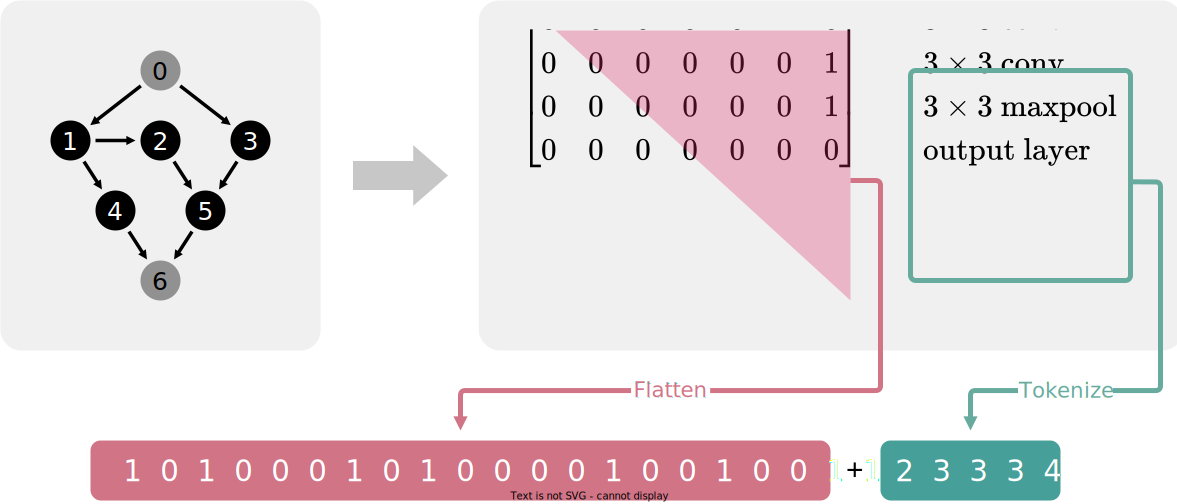
\includegraphics[width=.96\linewidth]{nb101-encoding}
  \caption{Illustration of tokenizing an OON architecture (from NAS-Bench-101) as a sequence.
    The symbol ``+'' represents concatenating two sequences.}\label{fig:nb101-encoding}
\end{figure}

\begin{figure}
  \centering
  \includegraphics[width=.98\linewidth]{vocabulary}
  \caption{
    The operator vocabularies for NAS-Bench-101, NAS-Bench-201 and DARTS space respectively.
  }\label{fig:vocabulary}
\end{figure}





\textbf{OOE Encoding.}\quad
In contrast to the OON encoding, the ``Operator On Edge'' encoding paradigm treats operators as edges and data as nodes.
This coding approach, exemplified by search spaces like that in DARTS~\cite{DBLP:conf/iclr/LiuSY19} and NAS-Bench-201~\cite{DBLP:journals/pami/DongLMG22}, facilitates the compression of both topological and operator information of the neural architecture into the adjacency matrix, leading to denser information representation regarding the relationships between operators and their interactions with data nodes.
A neural architecture cell \( \archOri=(A) \) containing \( n \) nodes will be coded as a sequence \( \mathrm{Tkn}_\mathrm{E}(\archOri) \) of length \( l_\mathrm{E}+2 \):
\begin{empheq}[left=\empheqlbrace]{equation}
  \begin{aligned}
     & \mathrm{Tkn}^{\mathstrut}_\mathrm{E} (\archOri) = \{\mathtt{CLS}\}\,\cup\,\underbracket[.5pt]{\mathrm{Triu} (A)}_\text{\( l^{\mathstrut}_\mathrm{E} \) tokens}\,\cup\,\{\mathtt{END}\} \\
     & l^{\mathstrut}_\mathrm{E} = \frac{n (n-1)}{2} = \frac{1}{2} (n^2-n)
  \end{aligned}
  \label{eq:ooe-tokenizer}
\end{empheq}
where the sequence is constructed by flattening the upper triangular arrays of adjacency matrices along with the inclusion of special tokens.
Specifically, in cases where diverse cell types exist within the neural architecture (\eg,\ DARTS search space), their sequences are seamlessly concatenated.
This concatenation strategy allows for the holistic representation of the entire architecture, considering the distinctive characteristics of each cell type within the unified sequence.


\begin{figure*}[t]
  \centering
  \includegraphics[width=.9\linewidth]{repr-learner}
  \caption{
    Illustration of the proposed representation learner.
    In the pre-training phase, only the neural architecture reconstruction loss is optimized, while the relative performance predictor (Ranker) is not involved in training.
    In the fine-tuning phase, reconstruction loss and prediction loss are jointly optimized.}\label{fig:repr-learner}
\end{figure*}

\subsubsection{Transformer-based Variational Auto-Encoder}

Given the nuanced nature of neural architecture, encompassing both structural and semantic information, we develop a neural architecture representation leveraging the Transformer~\cite{DBLP:conf/nips/VaswaniSPUJGKP17,DBLP:conf/cvpr/YiZH0023}, whose adeptness in handling sequences of variable lengths proves particularly advantageous for encoding the diverse architectures encountered in NAS\@.
Furthermore, the Transformer's capacity to capture global interactions across the input sequence offers a comprehensive understanding of the entire architecture, vital for discerning the intricate relationships between its components.
Consequently, the Transformer emerges as an ideal choice for our neural architecture representation, providing robustness, efficiency, and extensibility essential for effectively capturing the complexities of neural architectures.

The design of the representation learner is rooted in the VAE framework (as shown in Fig.~\ref{fig:repr-learner}), influenced by the pioneering work in the field~\cite{DBLP:conf/nips/YanZAZ020,DBLP:conf/ijcnn/LukasikFZHK21}, which facilitates bi-directional mapping between the architecture and representation spaces.
The selection of VAE is attributed to its several key advantages.
Primarily, the injective encoding property ensures the unique capture of local structural information, thereby guaranteeing distinct representations for each architecture while preserving rich structural details.
Moreover, VAEs promote the clustering of similar architectures within the latent space, thereby facilitating smooth architectural transitions.
This smooth latent space proves beneficial for downstream tasks, \eg, evaluating neural architectures, as similar architectures will produce close performance~\cite{Liu2020ASO}.
The neural architecture representation, thus, leverages these VAE properties to provide a comprehensive understanding of the complex structural relationships across different architectures.











Initially, the VAE encoder \( \encDist_{\encParam}(\archLtn|\archOri) \) parameterized by \( \encParam \) is employed to map the input data \( \archOri \), which consists of a finite number of independent identical distribution samples from an unknown distribution, to a continuous latent variable \( \archLtn \).
Following this encoding step, a probabilistic generative model \( \decDist_{\decParam}(\archOri|\archLtn) \), as known as the decoder, reconstructs the latent variables \( \archLtn \) back to their original representation.
The parameters \( \encParam \) and \( \decParam \) of the encoder and decoder, respectively, are optimized by maximizing
\begin{multline}\label{eq:vae-loss}
  \mathcal{L}_{\encParam,\decParam}{(\archOri)} = \mathbb{E}_{\archLtn \sim \encDist_{\encParam}(\archLtn|\archOri)}{\big[\log{\decDist_\decParam(\archOri|\archLtn)}\big]} \\
  {-}\: D_\mathrm{KL}\big(\encDist_\encParam(\archLtn|\archOri)\:||\:\decDist_\decParam(\archLtn)\big)
\end{multline}
where the first term is the \textit{Evidence Lower Bound} (ELBO), which represents the reconstruction loss, which ensures a high similarity between the input data and the data generated by the decoder and plays a crucial role in maintaining fidelity between the original and reconstructed data.
In contrast, the second term is the \textit{Kullback-Leibler Divergence} (KLD), serving as a regularization term for the latent space, which encourages the distribution of latent variables to remain close to the prior distribution, thus promoting a well-behaved and structured latent space.

The following outlines the specifications of the proposed Transformer-based VAE encoder and decoder models that are designed to effectively capture and reconstruct the complex structural relationships within neural architectures.

\textbf{Encoder.}\quad
For a given neural architecture \( \archOri \), it undergoes several transformations before input into the Transformer encoder.
Initially, the architecture is tokenized into a sequence of discrete tokens using Eq.~(\ref{eq:oon-tokenizer}) or Eq.~(\ref{eq:ooe-tokenizer}), each representing a specific architectural component or operation, to ensure the compatibility of the input with the Transformer encoder's format.
Subsequently, each token is mapped to a high-dimensional embedding vector using a learned embedding layer \( \mathrm{Emd}(\cdot) \), capturing semantic relationships between architectural components.
Positional embeddings \( E_\mathrm{pos} \) are then added to provide positional information, crucial for the Transformer Encoder to understand the order of architectural components, as illustrated in Eq.~(\ref{eq:enc-embedding}).











The resulting sequence of token embeddings, enriched with positional information, is fed into the Transformer encoder.
Here, the input undergoes processing through multi-head self-attention layer \( \mathrm{MSA}(\cdot) \) and feed-forward layer \( \mathrm{FF}(\cdot) \), yielding a contextualized representation of the neural architecture.
Layer normalization \( \mathrm{LN}(\cdot) \) is applied to the inputs of each layer, and the outputs are added to the residual connections, following the typical Transformer layer design. Formally, an architecture \( \archOri \) can be encoded using an \( \numLayer \)-layers Transformer-based architecture encoder \( \trmEnc(\cdot) \) as











\begin{empheq}[
    left={\trmEnc(\archOri)\Rightarrow \empheqlbrace}
  ]{alignat=2}
  % \begin{aligned}
  & \archHid^{(0)} & = {} & \mathrm{Emd} (\mathrm{Tkn} (\archOri)) + E_\mathrm{pos}\label{eq:enc-embedding}          \\
  & \archAtn^{(i)} & = {} & \mathrm{LN} (\mathrm{MSA} (\archHid^{(i-1)})) + \archHid^{(i-1)}                \notag{} \\
  & \archHid^{(i)} & = {} & \mathrm{LN} (\mathrm{FF} (\archAtn^{(i)})) + \archAtn^{(i)}                     \notag{}
  % & \archHid{}     & = {} & \mathrm{LN} (\archHid^{L}),
  % \end{aligned}
\end{empheq}
where \( i \in [1,\numLayer] \), \(\archHid^{(i)}\) and \(\archAtn^{(i)}\) represent the hidden states and attention states of the \(i\)-th layer, respectively.

Specifically, the hidden states of the \texttt{CLS} token are utilized as the memory of the input architecture sequence, and thus we can compute two representations
\begin{align}
  \archMem           & = \archHid^{(\numLayer)}[1,:]    \\
  \archRepr_{\mu}    & = \mathrm{FC}_{\mu}(\archMem)    \\
  \archRepr_{\sigma} & = \mathrm{FC}_{\sigma}(\archMem)
\end{align}
where \(\archMem\) represents the memory of the input architecture, while \(\archRepr_{\mu}\) and \(\archRepr_{\sigma}\) are the mean and variance of the distribution of learned neural architecture representations, respectively.
The two \( \mathrm{FC}(\cdot) \) represent fully-connected layers in the same settings. Thus, the outputs of our encoder are the parameters of the approximate posterior distribution
\begin{equation}
  \encDist_\encParam(\archLtn|\archOri) = \mathcal{N}(\archLtn;\archRepr_\mu,\varSigma),
\end{equation}
in which \( \varSigma = \archRepr_{\sigma}I \) acts as the variance-covariance matrix of the multi-variate normal distribution.

\textbf{Decoder.}\quad
The Transformer-based VAE decoder \( \decDist_{\decParam}(\archOri|\archLtn) \) takes a latent point \( \archLtn \) as input and reconstructs \( \archOri \).
To ensure optimal reconstruction stability, the original neural architecture \( \archOri \), which may have variable length, is reconstructed based on the reconstructed memory in the form of a causal prediction (Algorithm~\ref{algm:causal-predict}).
Utilizing a linear layer with activation functions, the reconstructed memory \( \archMem^\prime = \mathrm{ReLU}(\mathrm{FC}(\archLtn)) \) is obtained.
The reconstruction process commences with an initial sequence containing a {\texttt{CLS}} and recursively predicts the next token until the \texttt{END} token is encountered or until the sequence reaches its maximum length~\( L \).



\begin{equation}
  \trmDec(\rectOrig;\archMem^\prime)\Rightarrow\left\{
  \begin{alignedat}{2}
     & \rectVect^{(0)} & = {} & \mathrm{Emd} (\mathrm{Tkn} (\rectOrig)) + E_\mathrm{pos}                        \\
     & \rectStat^{(i)} & = {} & \mathrm{LN} (\mathrm{MSA} (\rectVect^{(i-1)})) + \rectVect^{(i-1)}              \\
     & \rectCond^{(i)} & = {} & \mathrm{LN} (\mathrm{MHA} (\archMem^\prime, \rectStat^{(i)})) + \rectStat^{(i)} \\
     & \rectVect^{(i)} & = {} & \mathrm{LN} (\mathrm{FF} (\rectCond^{(i)})) + \rectCond^{(i)}
    %  & \rectVect       & = {} & \rectVect^{(N)}[-1,:]
  \end{alignedat}\right.
\end{equation}
where \( i \in [1,\numLayer] \), \(\rectVect^{(i)}\) represents the hidden states of the \(i\)-th layer in the decoder.
\(\rectStat^{(i)}\) and \(\rectCond^{(i)}\) represent the intermediate states of multi-head self-attention.


\begin{algorithm}[tb]
  \caption{Architecture Causal Reconstruction}\label{algm:causal-predict}
  \SetAlgoLined{}
  \KwIn{Encoder memory \( \mathbf{m^\prime} \), Initial token \( y_0 \)}
  \KwOut{Complete output sequence \( \rectOrig \)}
  \BlankLine
  Initialize \( \rectOrig \gets \{y_0\} \)\;
  \BlankLine
  \For{\( t \gets 1 \) \KwTo \( T \)}{
    Decoder hidden state \( \rectVect_{t} \gets \trmDec(\rectOrig) \)\;
    Compute token probability distribution \( p(y_{t}|\mathbf{h}) \)\;
    Sample token \( y_t \) from \( p(y_t|\archHid) \)\;
    Append \( y_t \) to \( \rectOrig \)\;
    \lIf{\( y_t = \mathtt{END} \)}{break}
  }
  \BlankLine
  \Return{\( \rectOrig \)}\;
\end{algorithm}


\subsubsection{Incorporate Relative Performance Knowledge}

The primary objective here is to utilize the architecture's performance measure to establish mappings between representation spaces corresponding to different search spaces.
This facilitates the transfer of solutions across different domains, thereby improving the efficiency and effectiveness of the search process.
To enhance the learning process of neural architecture representations, we propose the incorporation of supervised signals related to architecture performance. Specifically, we employ a neural architecture performance predictor to swiftly evaluate a neural architecture or its representation.
The predictor serve to adjust the distribution of architecture representation, revealing features that are more oriented towards performance metrics. Furthermore, the predictor is utilized to construct mappings between the spaces of representations by efficiently providing the desired performance labels, enables the model to better understand the relationship between architectural representations and their corresponding performance, thereby guiding the search process towards high-performing solutions.

In line with the design of ReNAS~\cite{DBLP:conf/cvpr/Xu00TJX021}, we introduce a relativistic neural architecture performance predictor, comprising a multi-layer perceptron with activation functions.
Given that the evaluation strategy of NAS primarily focuses on discovering superior neural architectures rather than the specific performance of individual architectures, it is beneficial to relax the goal of performance prediction.
By concentrating on capturing the relative differences between architectural performances, the model can more effectively differentiate the ranking of neural architectures. Given a set of architecture representations \( Z = {\{ \archLtn^{i} \}}_{1}^{n} \), the relativistic predictor, a.k.a.\ ranker, can be trained by optimizing
\begin{gather}
  \begin{aligned}
    \Delta_{\mathrlap{\mathrm{pred}}}^{(i,j)}(Z) & = \predModel_{\predParam}(\archLtn^i) - \predModel_{\predParam}(\archLtn^j) \\
    \Delta_{\mathrlap{\mathrm{sign}}}^{(i,j)}(Z) & = \mathrm{Sign}(y_i-y_j)
  \end{aligned} \notag \\
  \mathcal{L}_\mathrm{rel} = \sum_{\mathclap{i=1}}^{n-1}{\;\sum_{\mathclap{j=i+1}}^{n}{\exp{\left( \Delta_\mathrm{pred}^{(i,j)}(Z) \times \Delta_\mathrm{sign}^{(i,j)}(Z)\right)}}}
\end{gather}
\noindent where \( \predModel_\predParam(\cdot) \) is the result of the performance predictor.
\(\Delta_{\mathrlap{\mathrm{pred}}}^{(i,j)}(Z)\) represents the difference in predicted performance, while \(\Delta_{\mathrlap{\mathrm{sign}}}^{(i,j)}(Z)\) measures the relative ranking between the true values of performance.

\subsubsection{Hybrid Supervised Training}

The construction of neural architecture representations involves a meticulous process that encompasses both unsupervised pre-training and supervised fine-tuning phases, each serving distinct yet complementary purposes in achieving robust and transferable representations.
\DiffAdd{During pre-training, the representation learner processes neural architectures from both source and target domains through encoding and decoding, establishing a foundational understanding of architectural patterns and features independent of performance metrics. The subsequent fine-tuning phase incorporates task-specific performance data to optimize representations for the target domain while maintaining transferability. This supervised phase calibrates the learned representations to align with domain-specific requirements and performance objectives.}

\DiffAdd{This dual-phase approach minimizes reliance on labeled data, which is especially valuable in new domains with limited performance measurements. The unsupervised pre-training enables broad recognition of architectural patterns, while fine-tuning ensures domain-specific optimization. Overall, the method strikes a balance between knowledge transfer and domain adaptation, facilitating efficient cross-domain knowledge transfer without compromising representation quality or task-specific relevance.}




\textbf{Unsupervised Pre-training.}\quad
Crucially, the pre-training phase operates under the premise of leveraging abundant unlabeled data to drive unsupervised learning processes, thereby circumventing the prohibitive costs associated with obtaining performance labels for neural architectures.
During this stage, the optimization objective predominantly revolves around minimizing the reconstruction loss, as the model endeavors to faithfully reconstruct architectural configurations from the representation space.
Based on Eq.~(\ref{eq:vae-loss}), the reconstruction and regularization losses can be described as follows:
\begin{align}
  \mathcal{L}_\mathrm{rec} & = \mathbb{E}_{\archLtn \sim \encDist_{\encParam}(\archLtn|\archOri)}{\big[\log{\decDist_\decParam(\archOri|\archLtn)}\big]}            \\
  \mathcal{L}_\mathrm{reg} & = {-}D^{\mathstrut}_\mathrm{KL}\big(\encDist_\encParam(\archLtn|\archOri)\:\|\:\decDist_\decParam(\archLtn)\big) \notag                \\
  {}                       & = {-}\frac{1}{2}\sum{\left({1+\log{(\archRepr^{\mathstrut}_{\sigma}) - \archRepr_{\mu}^{2} - \archRepr^{\mathstrut}_{\sigma}}}\right)}
\end{align}






In the pre-training stage of our framework, a notable feature is the deliberate inactivity of the relative performance predictor, or ranker.
This component remains dormant, abstaining from direct involvement in the training process.
Our approach employs a strategic decoupling of optimization objectives during this phase.
This methodology enables our model to learn generalizable features of neural architectures that are not tethered to domain-specific performance metrics.
The decoupling process facilitates the capture of intrinsic architectural characteristics, fostering a more versatile and transferable representation.
Consequently, this approach lays a robust foundation for subsequent cross-domain transfer tasks.
Formulary, the optimization object can be expressed as:
\begin{equation}
  \mathcal{L}_\mathrm{pt} = \mathcal{L}_\mathrm{rec} + \alpha\mathcal{L}_\mathrm{reg}
\end{equation}
where \(\alpha\) is a weight factor that balances the reconstruction and regularization losses.

\textbf{Supervised Fine-tuning.}\quad

In the fine-tuning phase, the neural architecture representation learner engages in a process of refinement, harnessing supervised learning techniques. This stage pivots towards a paradigm where labeled data, albeit scarce compared to the vast pool of unlabeled samples, serves as the cornerstone for honing the predictive capabilities of the representation mappings.
The fine-tuning process employs a joint optimization framework, where both reconstruction loss and prediction loss converge harmoniously. This convergence guides the model towards a point where the synthesized representations not only capture the structural intricacies of neural architectures but also exhibit adeptness in predicting their relative performance across diverse task domains.
This phase culminates in the emergence of finely calibrated neural architecture representations, poised to facilitate seamless knowledge transfer and domain adaptation across heterogeneous environments. The optimization process during this stage is encapsulated in the following objective function:



\begin{equation}
  \mathcal{L}_\mathrm{ft} = \mathcal{L}_\mathrm{rec} + \alpha\mathcal{L}_\mathrm{reg} + \beta\mathcal{L}_\mathrm{rel}
\end{equation}
where \(\mathcal{L}_\mathrm{rel}\) is the relative performance prediction loss, while hyperparameters \(\alpha\) and \(\beta\) control the balance between these components, allowing for fine-grained control over the learning process.





\subsection{Constructing Cross-Domain Representation Mapping}

Expanding upon the components of the previously mentioned architecture representation learner, NAS solutions can be explicitly transferred to tasks in other domains through the proposed \OUR{}.
As illustrated in Fig.~\ref{fig:overview}, the following steps focus on constructing a mapping between representation spaces of the source and the target domain, enabling the explicit transfer of neural architecture solutions across domains.
By establishing this mapping, the model can effectively leverage the knowledge gained from the source domain to improve the search process and discover high-performing architectures in the target domain.


Establishing a mapping between the representation spaces of source and target domains crucially facilitates knowledge transfer across domains.
Let \( \mathbb{R}^{\mathstrut}_{\mathcal{S}} \) and \( \mathbb{R}^{\mathstrut}_{\mathcal{T}} \) represent the representation spaces of the source (\( \mathcal{S} \)) and target (\( \mathcal{T} \)) domains, respectively.
The goal is to learn a mapping function \( \mathcal{M}: \mathbb{R}^{\mathstrut}_{\mathcal{S}} \rightarrow \mathbb{R}^{\mathstrut}_\mathcal{T} \) that minimizes the discrepancy between the mapped representations from the source domain and their corresponding counterparts in the target domain.
Formally, the objective function to be minimized can be expressed as:
\begin{equation}
  \mathcal{L}_\mathrm{map}(\mathcal{M}) = \sum_{i=1}^{N}{\ell\left(\mathcal{M}(\archLtn_{s}^{(i)}),\archLtn_{t}^{(i)}\right)}
\end{equation}
where \( \archLtn^{(i)}_{s} \in \mathbb{R}^{\mathstrut}_{\mathcal{S}} \) and \( \archLtn^{(i)}_{t} \in \mathbb{R}^{\mathstrut}_{\mathcal{T}} \) are the \( i \)-th sampled representations from the source and target domains, respectively, and sort according to the predicted values; \( N \) is the total number of sampled representation pairs; and \( \ell \) is a loss function quantifying the dissimilarity between the mapped source representation and the target representation.
The selection of the mapping function \( \mathcal{M} \) may vary based on the characteristics of the representation spaces and the desired flexibility and complexity of the mapping.
In this work, we exemplify the use of a linear mapping, \( \mathcal{M}(\archLtn_{s}) = \archLtn_{s}W + \bm{b} \), where \( W \) and \( \bm{b} \) are learnable parameters representing the weight matrix and bias vector, respectively.
Utilizing the \textit{Mean Squared Error}~(MSE) loss as \( \ell \), the mapping effectively learns to project representations from the source domain onto the target domain by optimizing the objective function:
\begin{equation}
  \min_{W,\mathbf{b}} \mathcal{L}_\mathrm{map}(\mathcal{M}) = \frac{1}{N}\sum_{i=1}^{N}{\left\|\archLtn_{t}^{(i)} - \left(\archLtn_{s}^{(i)}W + \bm{b}\right)\right\|}^{2}.
\end{equation}

\begin{algorithm}
  \SetAlgoLined{}
  \let\oldnl\nl % Store \nl in \oldnl
  \newcommand{\nonl}{\renewcommand{\nl}{\let\nl\oldnl}}% Remove line number for one line
  \caption{The proposed ESTO for \OUR{}}\label{algm:transfer}
  \KwIn{$P^{\mathstrut}_\mathrm{src}$, the set of solutions to be transferred obtained by a historical NAS process on the source domain; \(G\), the maximum generation count.}
  \KwOut{$P^{\mathstrut}_\mathrm{rst}$, the final population searched on the target domain.}

  \BlankLine{}

  \tcc{preparations}
  \( \big[\mathrm{Enc}^{\mathstrut}_{\mathcal{S}}(\cdot), \mathrm{Dec}^{\mathstrut}_{\mathcal{S}}(\cdot), \mathrm{Rkr^{\mathstrut}}_{\mathcal{S}}(\cdot)\big] \gets \) \\
  \nonl\hfill learning representations on source domain;

  \( \big[\mathrm{Enc}^{\mathstrut}_{\mathcal{T}}(\cdot), \mathrm{Dec}^{\mathstrut}_{\mathcal{T}}(\cdot), \mathrm{Rkr}^{\mathstrut}_{\mathcal{T}}(\cdot)\big] \gets \) \\
  \nonl\hfill learning representations on target domain;

  \(\mathcal{M} \gets \) learning mapping from \( \mathbb{R}^{\mathstrut}_{\mathcal{S}} \) to \( \mathbb{R}^{\mathstrut}_{\mathcal{T}} \)\;

  \BlankLine{}

  \tcc{sequential transfer}
  \( {R}^{\mathstrut}_\mathrm{src} \gets \mathrm{Enc}^{\mathstrut}_{\mathcal{S}} ({P}^{\mathstrut}_\mathrm{src}) \)\;
  % \( {R}^{\mathstrut}_\mathrm{trans} \gets \mathrm{Enc}^{\mathstrut}_{\mathcal{S}} ({P}^{\mathstrut}_\mathrm{trans}) \) \;
  % Map representations from source to target domain using mapping function $\mathcal{M}: \mathcal{R}_s \rightarrow \mathcal{R}_t$\;
  \( {R}^{\mathstrut}_\mathrm{tgt} \gets \mathcal{M}({R}^{\mathstrut}_\mathrm{src}) \)\;
  \( {P}^{\mathstrut}_{0} \gets \mathrm{Dec}^{\mathstrut}_{\mathcal{T}}({R}^{\mathstrut}_\mathrm{tgt}) \)\;

  \BlankLine{}

  \tcc{evolutionary NAS}
  \For{\( g \) from \( 1 \) to \( G \)}{
  % Apply evolutionary operations in target domain \;
  \( P^{\mathstrut}_\mathrm{new} \gets \) Apply evolutionary operations on \(P^{\mathstrut}_{g-1}\)\;
  \( F^{\mathstrut}_\mathrm{new} \gets \mathrm{Rkr}^{\mathstrut}_{\mathcal{T}}(P^{\mathstrut}_\mathrm{new}) \)\;
  \( P^{\mathstrut}_{g} \gets \) Binary tournament selection from \( P^{\mathstrut}_{g} \cup P^{\mathstrut}_{\mathrm{new}} \)\;
  }
  \( P^{\mathstrut}_\mathrm{rst} \gets P^{\mathstrut}_{g} \)\;

  \BlankLine{}

  \Return{\(P^{\mathstrut}_\mathrm{rst}\), the final population on target domain.}
\end{algorithm}

\subsection{Evolutionary TNAS with Cross-Domain Sequential Transfer}


Building on our cross-domain neural architecture mapping, we further design an ESTO algorithm --- a population-based approach capable of efficiently adapting the explicit transfer of solutions between domains.

\DiffAdd{
Our transfer method and solver are decoupled by design, allowing for the use of various solvers. However, we chose an evolutionary solver due to its distinct advantages. Firstly, evolutionary algorithms naturally maintain a diverse population of solutions, enabling the integration of transferred architectures while preserving exploration capabilities. This population-based approach offers more robust knowledge transfer than single-solution methods. Additionally, evolutionary crossover operations provide an effective mechanism for combining transferred knowledge with novel architectural patterns. This synergy allows the search process to leverage prior experience while uncovering new solutions specifically tailored to the target domain. Furthermore, evolutionary methods impose fewer constraints on the architecture representation, making them especially suitable for cross-domain transfer where source and target domains may differ in their search spaces.}


This approach leverages optimal neural architecture populations from the source domain to initialize and guide the evolutionary search process in the target domain, efficiently exploring promising regions in the target search space.
In the source domain, the framework first identifies the optimal neural architecture population using the pre-trained performance predictor. Top-performing individuals are selected to form an elite population, embodying the accumulated knowledge from the source domain.
The overview of the proposed ESTO algorithm in \OUR{} is presented in Algorithm~\ref{algm:transfer}. The process unfolds as follows:
\begin{itemize}
  \item \textbf{Knowledge Encoding (line 1--2):} The selected architectures from the optimal source population are encoded into representation vectors using the source domain's encoder. These encoded representations capture the essence of high-performing architectures discovered in the source domain.
  \item \textbf{Cross-Domain Mapping (line 3):} To transfer this knowledge to the target domain, the encoded representations are mapped from the source representation space to the target representation space using the learned mapping function \(\mathcal{M}\). This mapping operation effectively projects the optimal solutions from the source domain onto the target domain's architecture search space.
  \item \textbf{Initial Population Seeding (line 4--6):} The mapped representations in the target domain serve as the initial population for the evolutionary search process. This population, seeded with transferred knowledge from the source domain, provides a strategic starting point for the NAS to explore the target architecture search space.
  \item \textbf{Evolutionary Search (line 7--12):} The ESTO process then proceeds with a normal EA, but with a crucial difference --- the optimization is guided by the knowledge transferred from the source domain.
        % The performance predictor trained on the target domain \(\mathrm{Rkr}^{\mathstrut}_{\mathcal{T}}(\cdot)\) is used to evaluate the fitness of new architectures, ensuring that the search is tailored to the target domain's characteristics.
        The performance predictor, \(\mathrm{Rkr}^{\mathstrut}_{\mathcal{T}}(\cdot)\), trained on the target domain, is employed to assess the fitness of new architectures, ensuring the search is specifically adapted to the characteristics of the target domain.
        % \item Selection and Iteration: Through multiple generations, the population evolves using binary tournament selection, consistently improving the quality of architectures with respect to the target domain's objectives.
\end{itemize}











A critical consideration in transfer learning involves addressing the challenge of negative transfer – the fundamental mismatch between transferred knowledge and target task requirements. The proposed \OUR{} integrates multiple structural mechanisms to mitigate this phenomenon. First, our evolutionary optimization strategy preserves population diversity throughout the search process through three key design features: (1) The population-based paradigm maintains exploration capacity even when partial transferred solutions underperform, enabling recovery through subsequent evolutionary operations; (2) A transfer probability parameter regulates the proportion of transferred knowledge in initial populations, ensuring balanced exploitation of prior knowledge while preserving novel solution discovery in the target domain; (3) An adaptive selection mechanism rigorously evaluates transferred architectures against target task objectives, systematically eliminating suboptimal candidates during the evolutionary cycle.

By integrating EA with cross-domain transfer capabilities, \OUR{} effectively leverages existing NAS solutions and knowledge from diverse search spaces, potentially leading to more efficient and effective neural architecture search in new domains.

\end{document}